\documentclass{article} % For LaTeX2e
\usepackage{nips15submit_e,times}
\usepackage{hyperref}
\usepackage{url}
\usepackage{lineno}
\usepackage{graphicx}
\usepackage{amsmath}
\usepackage{multicol}
%\usepackage[all]{hypcap} 
\usepackage{listings}
\usepackage{float}
\usepackage{amsfonts}
\usepackage{multicol}
\usepackage{breqn}
\usepackage{bm}
\setlength{\columnsep}{1cm}
%\linenumbers% Uncomment for line numbers



\title{America's Warzone: Modeling Armed Robberies in Chicago}

\author{
Reuben K. McCreanor\thanks{Department of Statistical Science, Duke University} \\  
\texttt{reuben.mccreanor@duke.edu} \\
\And
Anna K. Yanchenko\footnotemark[1] \\
\texttt{anna.yanchenko@duke.edu} \\
\And 
Lei Qian\footnotemark[1] \\
\texttt{lei.qian@duke.edu} \\
\And
Megan S. Robertson\footnotemark[1] \\
\texttt{megan.robertson@duke.edu} \\ 
}

\hypersetup{
    colorlinks=true,
    linkcolor=blue,
    filecolor=magenta,      
    urlcolor=cyan,
    pdftitle={Sharelatex Example},
    bookmarks=true,
    pdfpagemode=FullScreen,
}


\newcommand{\fix}{\marginpar{FIX}}
\newcommand{\new}{\marginpar{NEW}}

\nipsfinalcopy 

\begin{document}

\maketitle

\section{Introduction}
\label{headings}

\noindent The city of Chicago is frequently listed as one of the most dangerous and crime-ridden cities in the US. President Donald Trump frequently discusses the high-rate of crime in Chicago. According to the Chicago Tribune, there were 4,367 shooting victims in Chicago in 2016. In the same year there were also 785 homicides.\hyperlink{Ref2}{[2]} However, other reports conclude that Chicago should not be called the crime capital�� of America, as Chicago's violence rate is lower than cities like St.  Louis and Detroit. \hyperlink{Ref1}{[1]} The goal of this project was to examine crime in Chicago, specifically armed robberies, from 2012-2016. \newline

\section{Data}
\label{headings}

\noindent The crime data used for this project came from the City of Chicago's website. \footnote{Crimes 2001 to present, \url{https://data.cityofchicago.org/Public-Safety/Crimes-2001-to-present/ijzp-q8t2/data}} The data contained every reported crime in Chicago from 2001 to the present (\autoref{data}). In addition to the type of crime reported (battery, assault, etc.), there was information on the location and time of the crime. The data set was reduced to only consider armed robberies. 

\begin{figure}[h]
\begin{center}

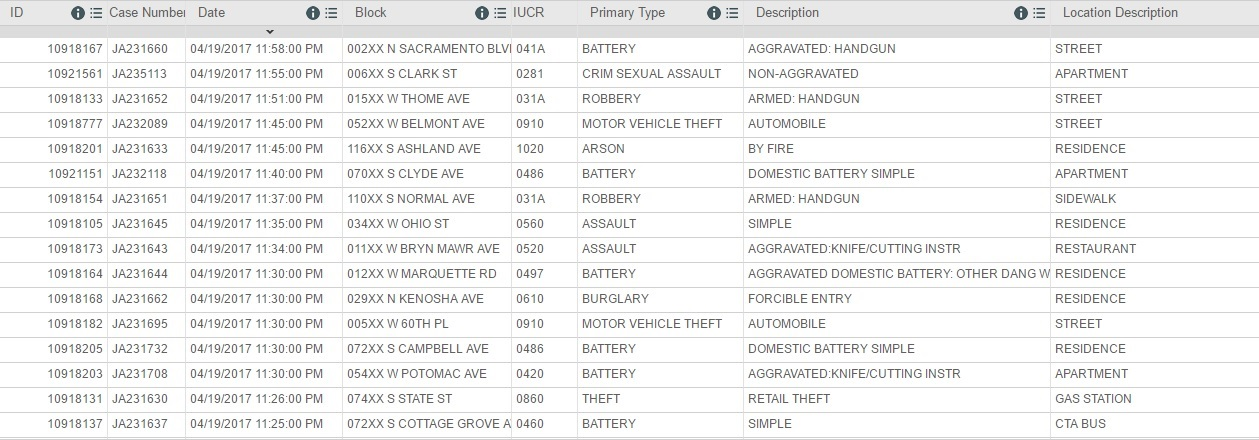
\includegraphics[width=0.8\textwidth,keepaspectratio]{data.jpg}
\caption{The city of Chicago website provides a data set containing information on crimes committed in the city from 2001 to present day.}
\label{data}
\end{center}
\end{figure}


\section{Time Series Analysis}


\noindent The city of Chicago is divided into regions known as sides (\autoref{sides}), where each side is comprised of several neighborhoods. There is a lot of variation in the population (\autoref{population}) and the number of armed robberies per capita (\autoref{counts}) for these sides.  Additionally, some sides are more residential, while others are more commercial.\newline
 
\begin{figure}[h]
\begin{center}

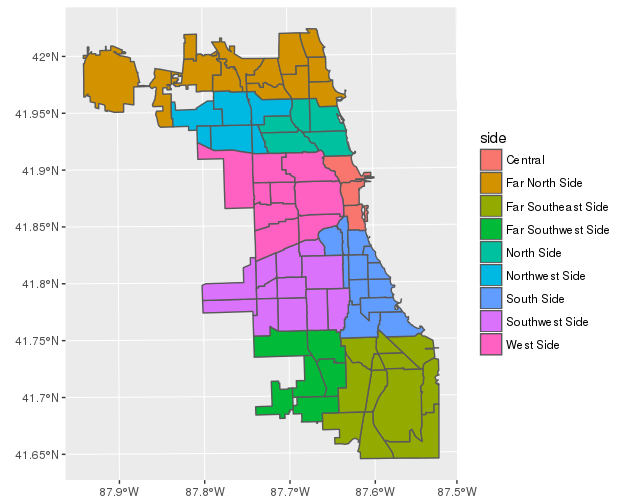
\includegraphics[width=0.8\textwidth,keepaspectratio]{CopyOfside.png}
\caption{The ``sides" of Chicago.  The borders correspond to  the boundaries of the community areas colored by the side.}
\label{sides}
\end{center}
\end{figure}


\begin{figure}[h]
\begin{center}

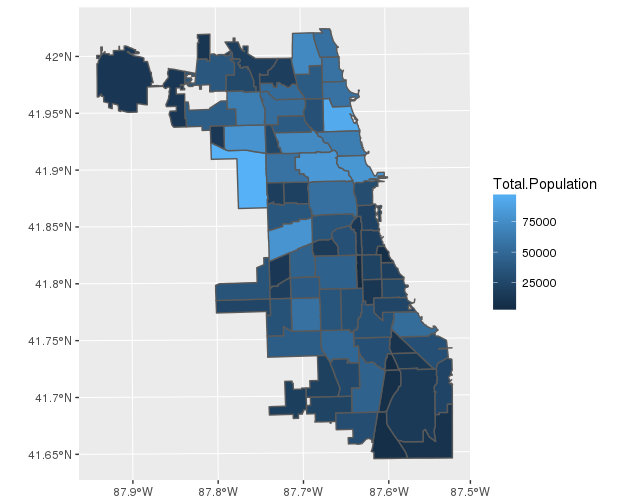
\includegraphics[width=0.8\textwidth,keepaspectratio]{Plots/population.png}
\caption{The population distribution of the  ``sides" of Chicago.  The borders correspond to  the boundaries of the community areas colored by the side.}
\label{population}
\end{center}
\end{figure}

\begin{figure}[h]
\begin{center}

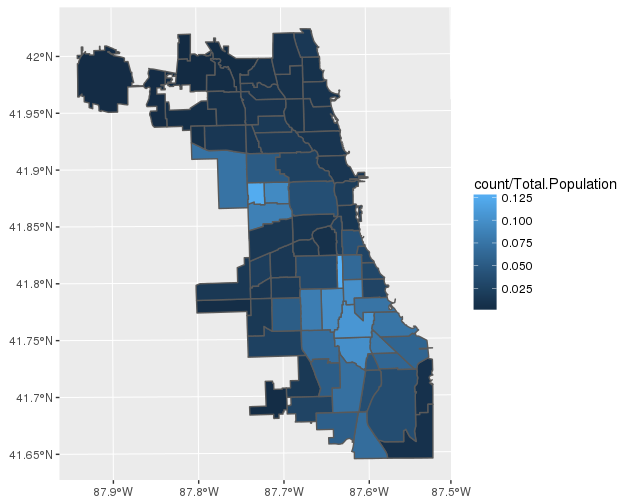
\includegraphics[width=0.8\textwidth,keepaspectratio]{Plots/counts_by_pop.png}
\caption{The number of armed robberies per capita for the ``sides" of Chicago between 2003 and 2016.  The borders correspond to  the boundaries of the community areas colored by the side.}
\label{counts}
\end{center}
\end{figure}

\noindent ARIMA models were fit to predict the counts of monthly armed robberies in each side of the city between 2003 and 2016. In order to determine the type of model, the ACF and PACF plots were examined for the data for each of the sides. For example, if there was structure in the PACF plot beyond one lag, moving average terms were added. The model residuals were also examined to ensure that there was no remaining structure in the residuals. The PACF and ACF plots for the data from the South Side are displayed below. The ACF plot showed evidence of seasonality at lag 12 (i.e. yearly trends). After lag 1, there was no large values for the PACF, so no moving average terms were included in the model. \newline

\break 
\begin{multicols}{2}
\begin{figure}[H]
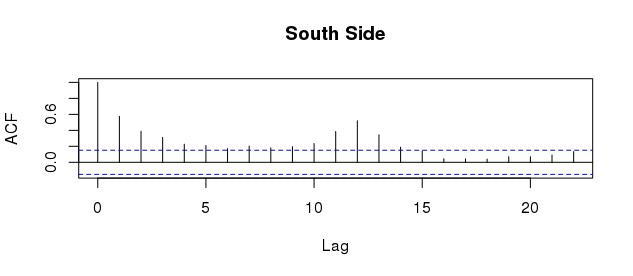
\includegraphics[width=70mm]{Plots/south_ACF.png}
\caption{ACF plot for the number of monthly armed robberies in the South Side of Chicago between 2003 and 2016.}
\end{figure}

\begin{figure}[H]
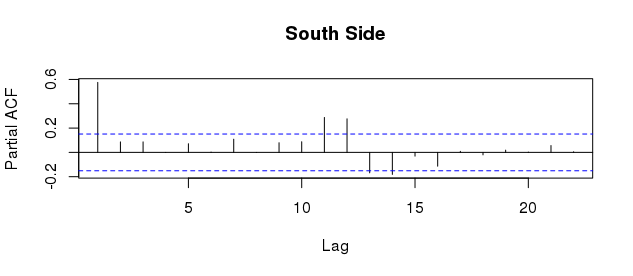
\includegraphics[width=70mm]{Plots/south_PACF.png}
\caption{PACF plot for the number of monthly armed robberies in the South Side of Chicago between 2003 and 2016.}
\end{figure}
\end{multicols}

\noindent Based on the ACF \autoref{south_resid_ACF} and PACF \autoref{south_resid_PACF} plots, an AR(4) model was fit with a seasonal component with period twelve. The residuals plot for this model did not display any remaining structure in the data and the coefficients are in \autoref{south_coef}. 

\begin{multicols}{2}
\begin{figure}[H]
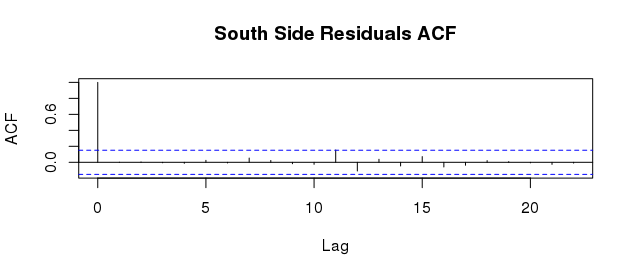
\includegraphics[width=70mm]{Plots/south_resid_ACF.png}
\caption{ACF plot of the residuals of an AR(4) model with a period twelve seasonal component fit to the monthly count of armed robberies for the South Side.}
\label{south_resid_ACF}
\end{figure}

\begin{figure}[H]
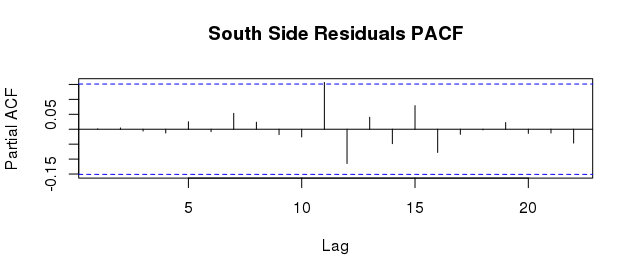
\includegraphics[width=70mm]{Plots/south_resid_PACF.png}
\caption{PACF plot of the residuals of an AR(4) model with a period twelve seasonal component fit to the monthly count of armed robberies for the South Side.}
\end{figure}
\label{south_resid_PACF}
\end{multicols}


 \begin{table}[h!]
\centering
\begin{tabular}{|p{2.3cm}|c| c|c|c|c|} 
 \hline
 & ar1 &    ar2 &    ar3 &    ar4 &   sar1 \\ [0.5ex] 
 \hline\hline
Coefficient & 0.3850 & 0.1328 & 0.0825  &0.0167 & 0.4784  \\\hline
Standard Error &   0.0793 & 0.0832&  0.0824 & 0.0771  &0.0708   \\
 \hline
\end{tabular}
\caption{Summary of model fit for the AR(4) with period 12 seasonal component fit to the monthly count of armed robberies for the South Side.}
\label{south_coef}
\end{table}

\noindent The coefficient estimates for all of the different sides were very similar.  While some sides displayed evidence of higher order autoregressive structure or the addition of moving average terms, as compared to the South Side, all sides had a clear period 12 seasonal component, indicating strong yearly trends for all sides of the city.  The coefficient estimates were positive for the autoregressive terms, indicating that there was a positive correlation between the amount of monthly armed robberies over time.  Plots of the various model fits can be found in \autoref{appendix_regression}.  It is interesting that although the sides of Chicago are quite diverse in terms of population and demographics, as well as the number of monthly armed robberies, the temporal trends for all of the sides are very similar.  Although the count of the monthly armed robberies differs by side of the city, the overall temporal trend is the same across Chicago and has a strong yearly, autoregressive trend.\newline   

\section{Spatial Models}





\newpage


\subsubsection*{References}


\hypertarget{Ref1}{[1]} Papachristos, Andrew V., "48 Years of Crime in Chicago: An Analysis of of Serious Crime Trends from 1965-2013,\url{http://isps.yale.edu/sites/default/files/publication/2013/12/48yearsofcrime_final_ispsworkingpaper023.pdf}, December 2013.

\hypertarget{Ref2}{[2]} Pearson, Rick, "Trump Again Assails Chicago gun violence in speech to Congress", \textit{Chicago Tribune}, \url{http://www.chicagotribune.com/news/local/politics/ct-donald-trump-congress-speech-chicago-met-20170228-story.html}, March 2017.


\clearpage
\newpage

\section{Appendix}
\label{appendix}


\subsection{Time Series Modeling Plots}
\label{appendix_regression}

 
\subsubsection{West Side}
 
\begin{multicols}{2}
 \begin{figure}[H]
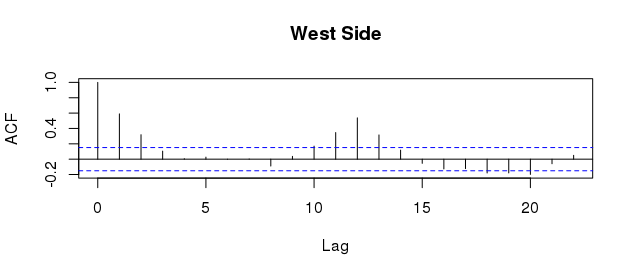
\includegraphics[height=50mm, width=80mm]{Plots/West_ACF.png}
\end{figure}
 
\begin{figure}[H]
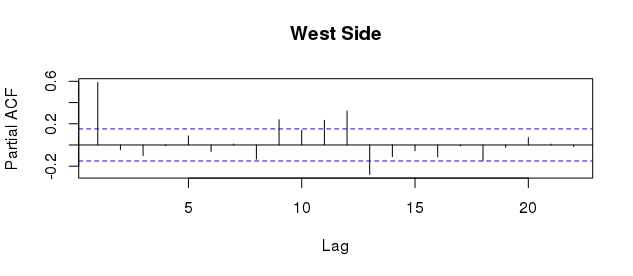
\includegraphics[height=50mm, width=80mm]{Plots/West_PACF.png}
\end{figure}
 
\begin{figure}[H]
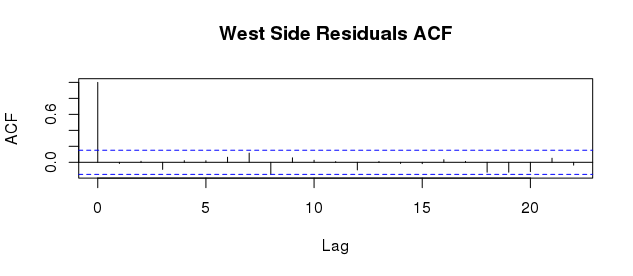
\includegraphics[height=50mm, width=80mm]{Plots/west_resids_ACF.png}
\end{figure}
 
\begin{figure}[H]
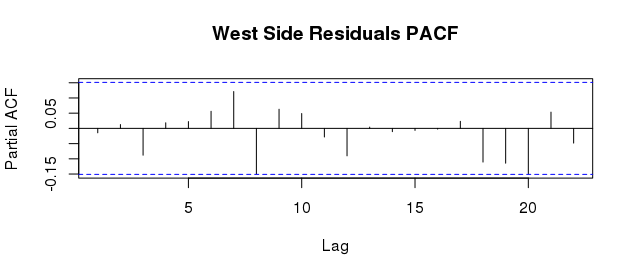
\includegraphics[height=50mm, width=80mm]{Plots/west_resids_PACF.png}
\end{figure}
 \end{multicols}
 
\begin{center}
\begin{figure}[H]
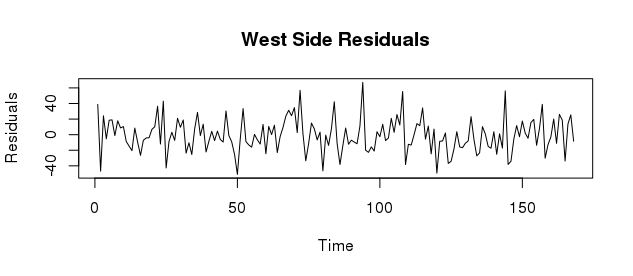
\includegraphics[height=50mm, width=80mm]{Plots/west_resids.png}
\end{figure}
\end{center}
 

 
\subsubsection{Southwest Side}
 
\begin{multicols}{2}
 
\begin{figure}[H]
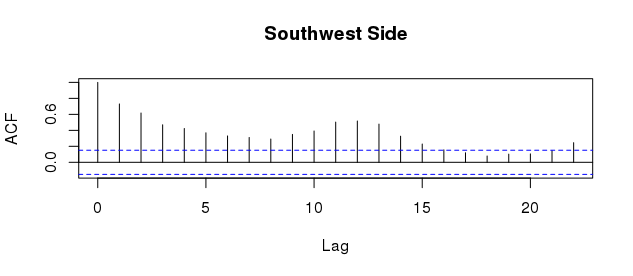
\includegraphics[height=50mm, width=80mm]{Plots/southwest_acf.png}
\end{figure}
 
\begin{figure}[H]
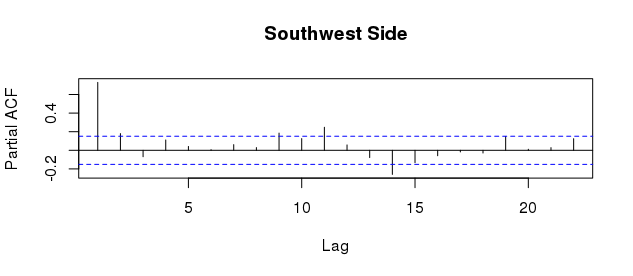
\includegraphics[height=50mm, width=80mm]{Plots/southwest_PACF.png}
\end{figure}
 
\begin{figure}[H]
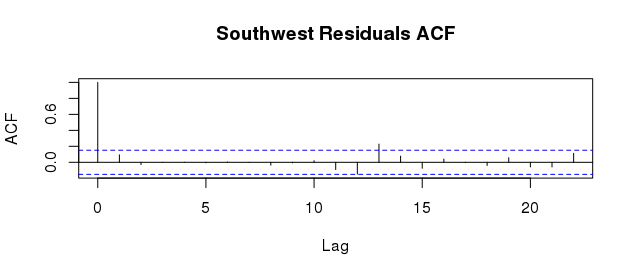
\includegraphics[height=50mm, width=80mm]{Plots/southwest_resid_ACF.png}
\end{figure}
 
\begin{figure}[H]
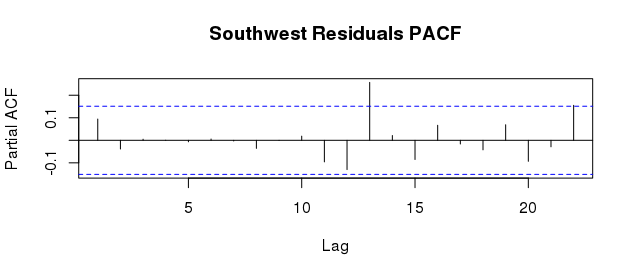
\includegraphics[height=50mm, width=80mm]{Plots/southwest_resid_pacf.png}
\end{figure}
 
\end{multicols}
 
\begin{center}
\begin{figure}[H]
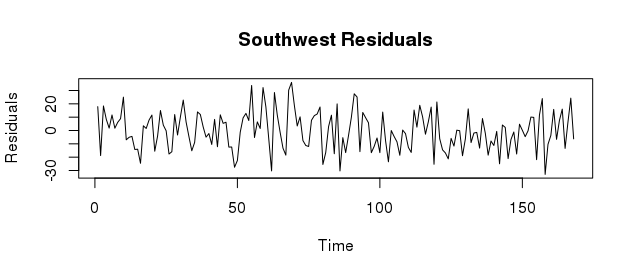
\includegraphics[height=50mm, width=80mm]{Plots/southwest_resid.png}
\end{figure}
\end{center}
 
 
\subsubsection{Southeast Side}
 
\begin{multicols}{2}
 
\begin{figure}[H]
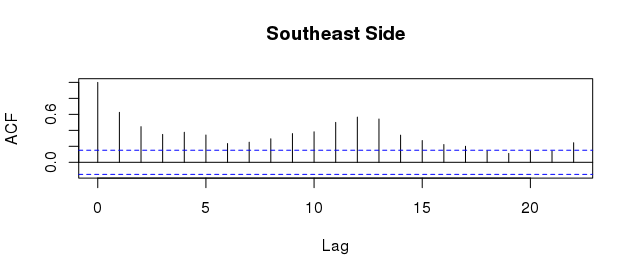
\includegraphics[height=50mm, width=80mm]{Plots/southeast_acf.png}
\end{figure}
 
\begin{figure}[H]
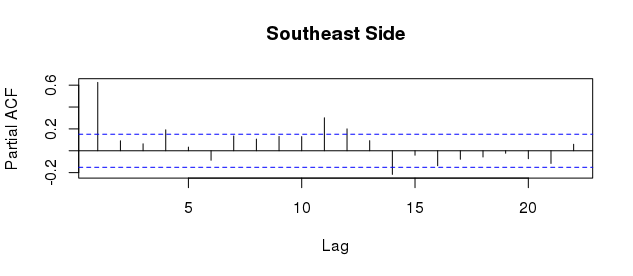
\includegraphics[height=50mm, width=80mm]{Plots/southeast_PACF.png}
\end{figure}
 
\begin{figure}[H]
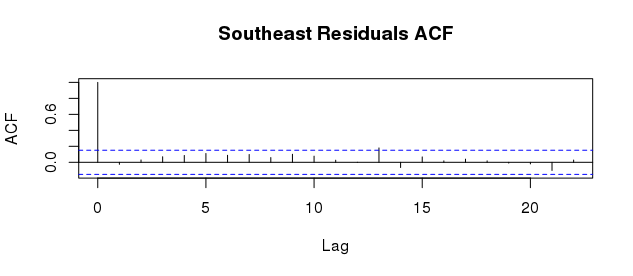
\includegraphics[height=50mm, width=80mm]{Plots/southeast_resid_acf.png}
\end{figure}
 
\begin{figure}[H]
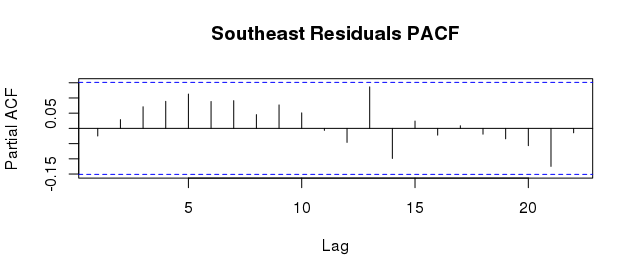
\includegraphics[height=50mm, width=80mm]{Plots/southeast_resid_pacf.png}
\end{figure}
 
\end{multicols}
 
\begin{center}
\begin{figure}[H]
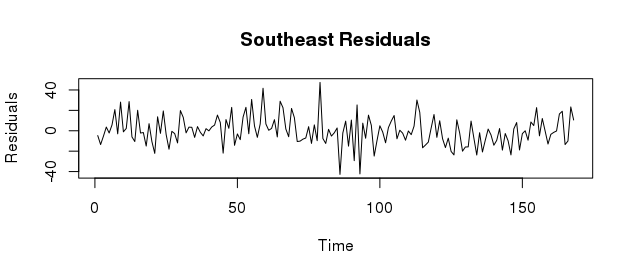
\includegraphics[height=50mm, width=80mm]{Plots/southeast_resid.png}
\end{figure}
\end{center}
\end{document}
 
 
\subsubsection{Northwest Side}
 
\begin{multicols}{2}
 \begin{figure}[H]
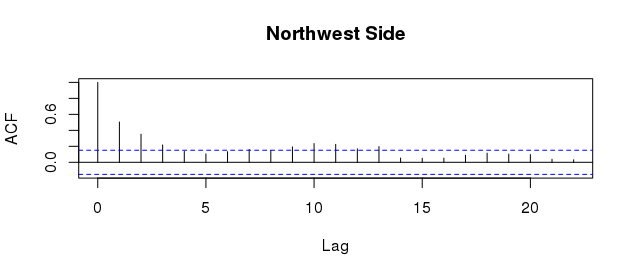
\includegraphics[height=50mm, width=80mm]{Plots/northwest_ACF.png}
\end{figure}
 
\begin{figure}[H]
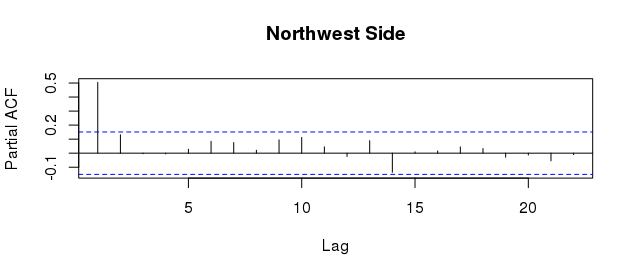
\includegraphics[height=50mm, width=80mm]{Plots/northwest_PACF.png}
\end{figure}
 
\begin{figure}[H]
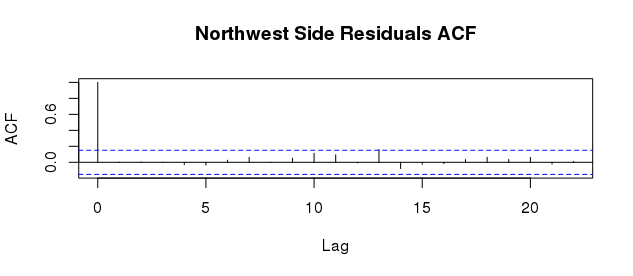
\includegraphics[height=50mm, width=80mm]{Plots/northwest_resid_ACF.png}
\end{figure}
 
\begin{figure}[H]
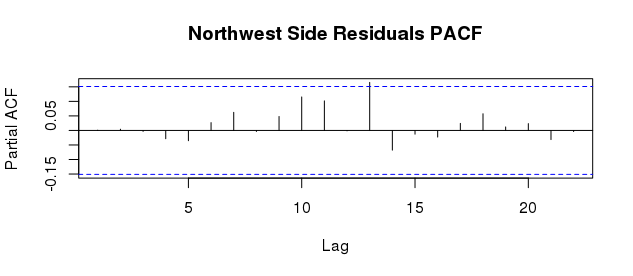
\includegraphics[height=50mm, width=80mm]{Plots/northwest_resid_PACF.png}
\end{figure}
 \end{multicols}
 
\begin{center}
\begin{figure}[H]
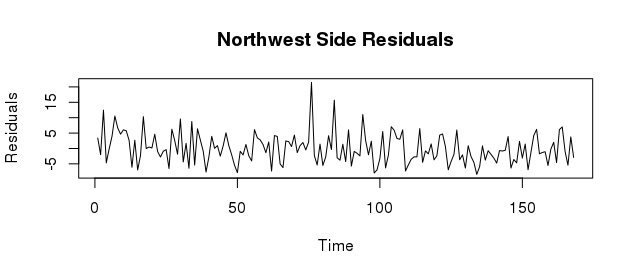
\includegraphics[height=50mm, width=80mm]{Plots/northwest_resids.png}
\end{figure}
\end{center}
 

 
\subsubsection{North Side}
 
\begin{multicols}{2}
 \begin{figure}[H]
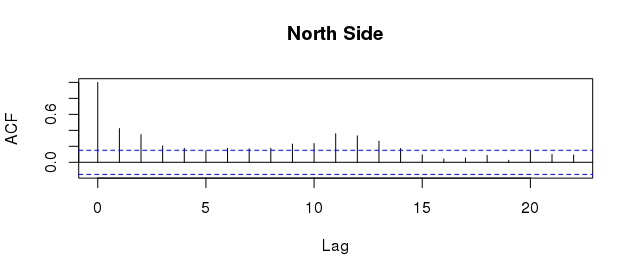
\includegraphics[height=50mm, width=80mm]{Plots/north_ACF.png}
\end{figure}
 
\begin{figure}[H]
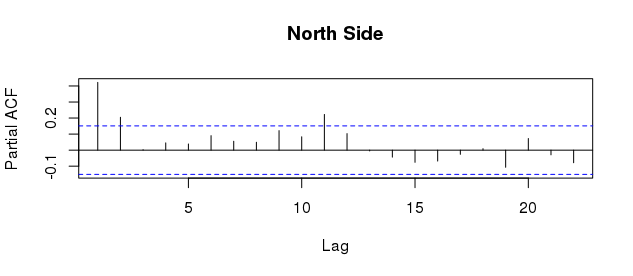
\includegraphics[height=50mm, width=80mm]{Plots/North_PACF.png}
\end{figure}
 
\begin{figure}[H]
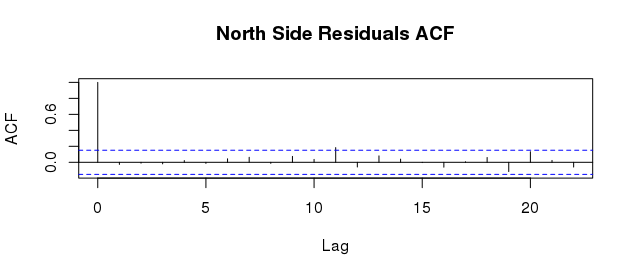
\includegraphics[height=50mm, width=80mm]{Plots/north_resid_ACF.png}
\end{figure}
 
\begin{figure}[H]
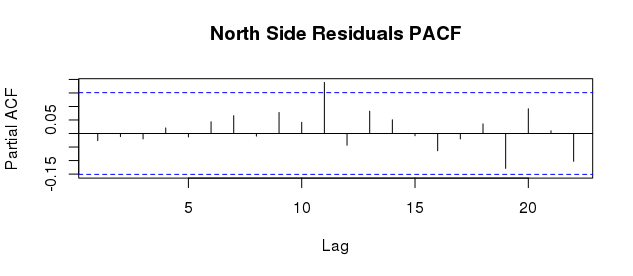
\includegraphics[height=50mm, width=80mm]{Plots/north_resid_PACF.png}
\end{figure}
 \end{multicols}
 
\begin{center}
\begin{figure}[H]
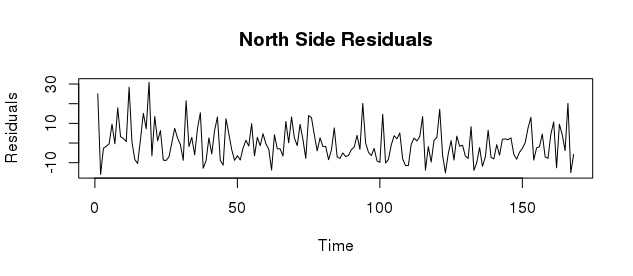
\includegraphics[height=50mm, width=80mm]{Plots/north_residuals.png}
\end{figure}
\end{center}
 

 
\subsubsection{Far Southwest Side}
\begin{multicols}{2} 
\begin{figure}[H]
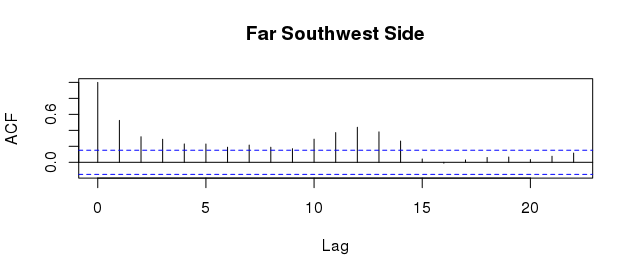
\includegraphics[height=50mm, width=80mm]{Plots/far_southwest_acf.png}
\end{figure}
 
\begin{figure}[H]
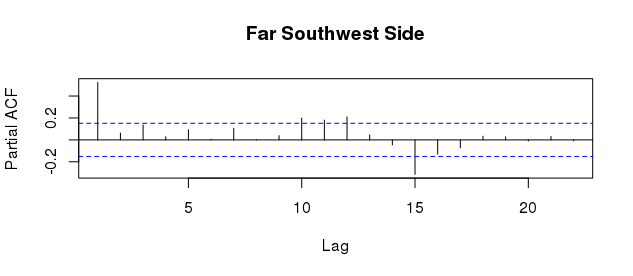
\includegraphics[height=50mm, width=80mm]{Plots/far_southwest_pacf.png}
\end{figure}
 
\begin{figure}[H]
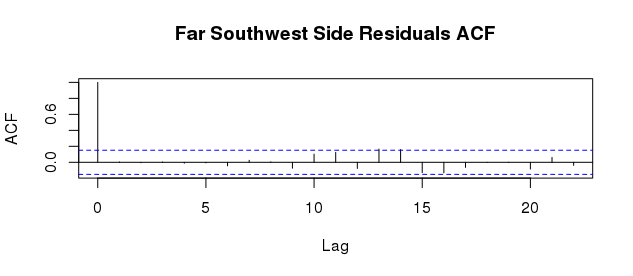
\includegraphics[height=50mm, width=80mm]{Plots/far_southwest_resid_acf.png}
\end{figure}
 
\begin{figure}[H]
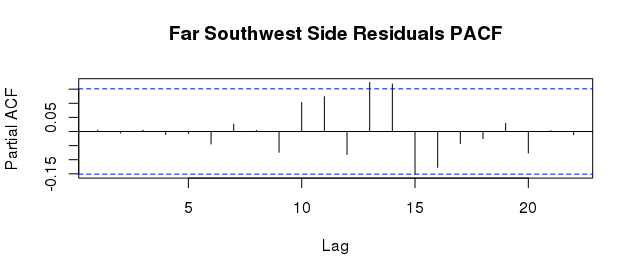
\includegraphics[height=50mm, width=80mm]{Plots/far_southwest_resid_pacf.png}
\end{figure}
 
\end{multicols}
 
\begin{center}
\begin{figure}[H]
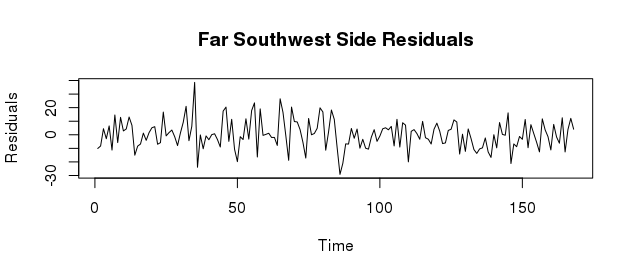
\includegraphics[height=50mm, width=80mm]{Plots/far_southwest_resid.png}
\end{figure}
\end{center}
 

 
\subsubsection{Far North Side}
 
\begin{multicols}{2} 
\begin{figure}[H]
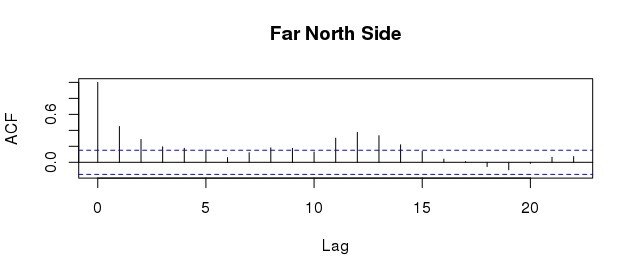
\includegraphics[height=50mm, width=80mm]{Plots/far_north_ACF.png}
\end{figure}
 
\begin{figure}[H]
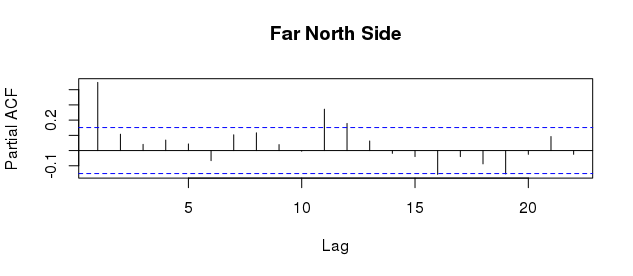
\includegraphics[height=50mm, width=80mm]{Plots/far_north_PACF.png}
\end{figure}
 
\begin{figure}[H]
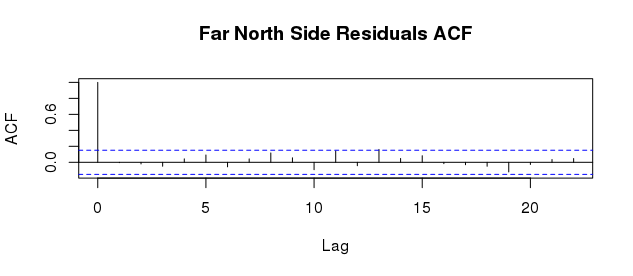
\includegraphics[height=50mm, width=80mm]{Plots/far_north_resids_ACF.png}
\end{figure}
 
\begin{figure}[H]
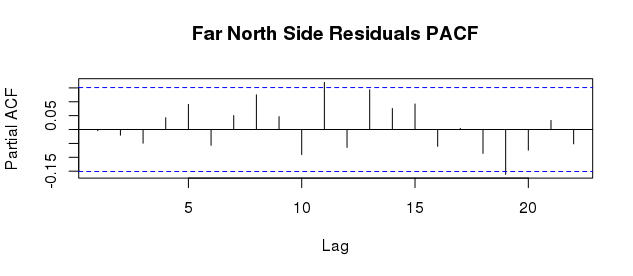
\includegraphics[height=50mm, width=80mm]{Plots/far_north_resids_PACF.png}
\end{figure}
 \end{multicols}
 
\begin{center}
\begin{figure}[H]
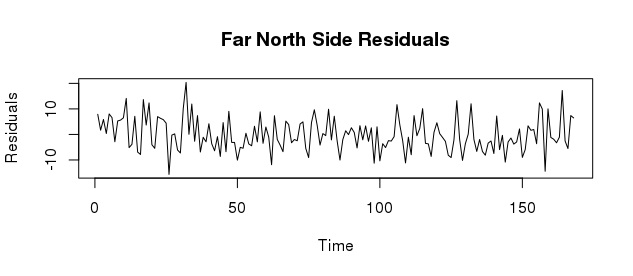
\includegraphics[height=50mm, width=80mm]{Plots/far_north_resids.png}
\end{figure}
 \end{center}
 

 
\subsubsection{Central}
 \begin{multicols}{2}
\begin{figure}[H]
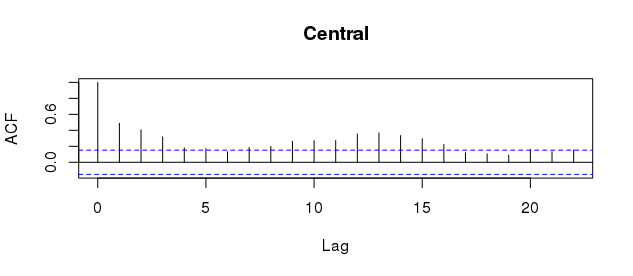
\includegraphics[height=50mm, width=80mm]{Plots/Central_ACF.png}
\end{figure}
 
\begin{figure}[H]
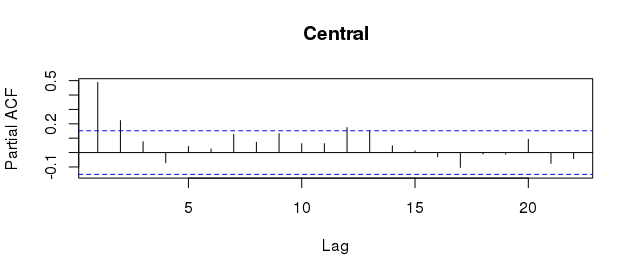
\includegraphics[height=50mm, width=80mm]{Plots/Central_PACF.png}
\end{figure}
 
\begin{figure}[H]
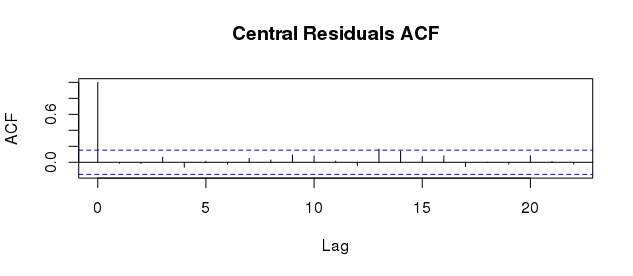
\includegraphics[height=50mm, width=80mm]{Plots/Central_resid_ACF.png}
\end{figure}
 
\begin{figure}[H]
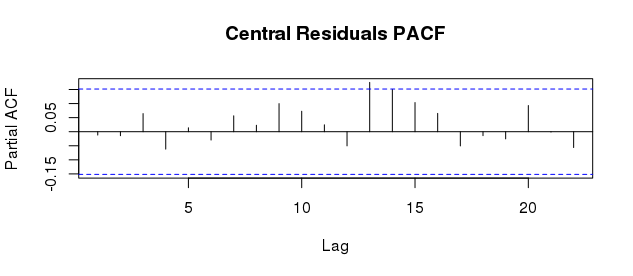
\includegraphics[height=50mm, width=80mm]{Plots/Central_resid_PACF.png}
\end{figure}
 \end{multicols}
 
\begin{center}
\begin{figure}[H]
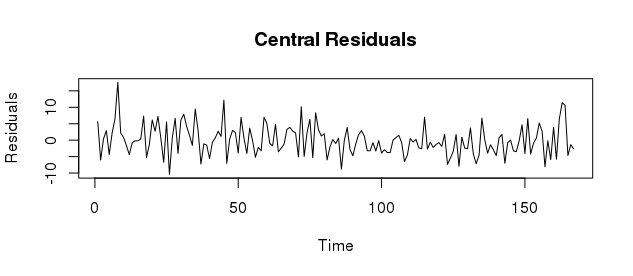
\includegraphics[height=50mm, width=80mm]{Plots/Central_residuals.png}
\end{figure}

\end{document}


